%++++++++++++++++++++++++++++++++++++++++
% Don't modify this section unless you know what you're doing!
\documentclass[letterpaper,12pt]{article}
\usepackage[utf8]{inputenc}
\usepackage{float}
\usepackage{tabularx} % extra features for tabular environment
\usepackage{amsmath}  % improve math presentation
\usepackage{graphicx} % takes care of graphic including machinery
\usepackage[margin=1in,letterpaper]{geometry} % decreases margins
\usepackage{cite} % takes care of citations
\usepackage[final]{hyperref} % adds hyper links inside the generated pdf file
\usepackage[table,xcdraw]{xcolor}
\hypersetup{
	colorlinks=true,       % false: boxed links; true: colored links
	linkcolor=blue,        % color of internal links
	citecolor=blue,        % color of links to bibliography
	filecolor=magenta,     % color of file links
	urlcolor=blue         
}
%++++++++++++++++++++++++++++++++++++++++


\begin{document}

\title{Práctica 3 - Ruteo}
\author{Matthew Aguerreberry, Natasha Tomattis}
\date{\today}
\maketitle

% \begin{abstract} 
% \end{abstract}


\section{Practica de Ruteo - OSPF}
	\begin{figure}[ht] 
			
		\centering 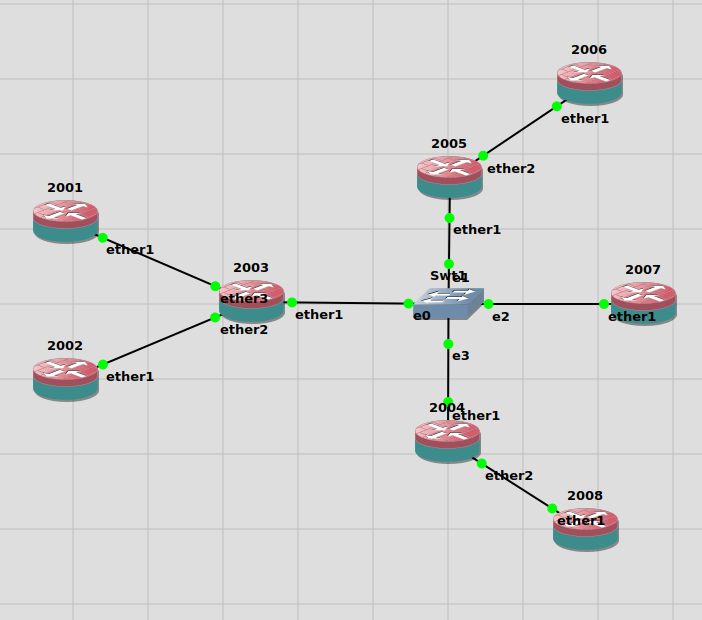
\includegraphics[width=0.8\columnwidth]{figure/topo_figura1.png}
		%\includegraphics[width=1.0\columnwidth]{sr_setup.pdf}
		\caption{
				\label{fig:samplesetup} % spaces are big no-no 
				Implementación Ejercicio 1.
		}
	\end{figure}
	\begin{enumerate}
		\item \textbf{Conectar los routers, switchs y nodos segun el diagrama de la figura 1.}
		\item \textbf{Configurar interfaces de acuerdo al diagrama.}
		\item \textbf{¿Configurar OSPF en todas los routers respetando las areas segun el diagrama. Es posible alcanzar todas las redes?} \\
		Si, todas las redes son compartidas a traves de OSPF.
		\item \textbf{Los routers de las areas no backbone, conocen todas las rutas a las demas redes?}\\
		Si, la division de areas no limita la propagacion de rutas OSPF.
		\item \textbf{Observando el área backbone, que router fue elegido como DR y cual como BDR? ¿Por qué fueron elegidos esos routers?}\\
		Se eligio el router con la router id más alto de la red 10.0.10.0/24 como DR y el subsiguiente como BDR. El router ID, por defecto, toma el valor de IP más bajo de las interfaces activas del dispositivo.
		\item \textbf{Elegir uno de los routers que no cumple una de esas funciones y configurarlo para que sea DR (no debe modificar el direccionamiento) ¿De qué manera/s puede hacer esto? Seleccione una para lograr lo solicitado.}\\
		Esto se puede lograr de varias maneras, por un lado se puede cambiar la prioridad del router la cual sera utilizada a la hora de la eleccion del DR; por otro lado se puede modificar el router-id ya sea a traves de la configuracion explicita de este parametro o la configuracion de una interfaz loopback con una direccion de mayor valar que los otros router-id. En nuestro caso configuramos una interfaz loopback1 en el dispositivo 2003 para que esta sea utilizada como router-id, como se puede ver en la imagen a continuacion.
		\begin{figure}[H] 
			
			\centering 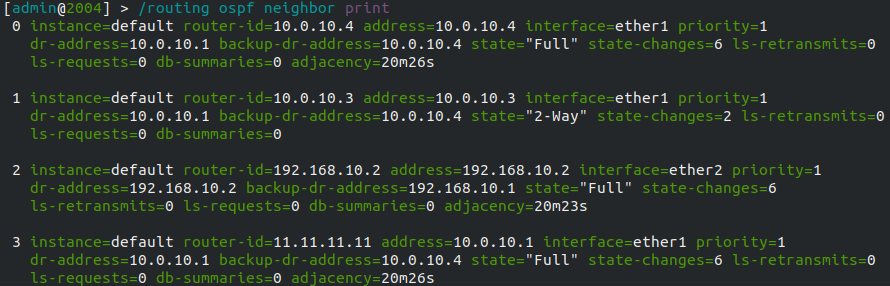
\includegraphics[width=0.5\columnwidth]{figure/int_loopback.png}
			%\includegraphics[width=1.0\columnwidth]{sr_setup.pdf}
			\caption{
					\label{fig:samplesetup} % spaces are big no-no 
					Configuracion de la interfaz loopback en el router 2003.
			}
		\end{figure} 
		\begin{figure}[H] 
			
			\centering 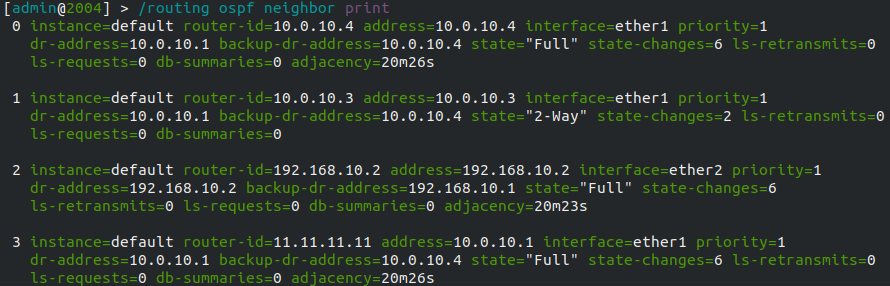
\includegraphics[width=0.8\columnwidth]{figure/new_dr.png}
			%\includegraphics[width=1.0\columnwidth]{sr_setup.pdf}
			\caption{
					\label{fig:samplesetup} % spaces are big no-no 
					Seleccion de la IP configurada en loopback como roter-id. Eleccion de nuevo DR.
			}
		\end{figure} 
		
	\end{enumerate}

	\subsection{Enlaces consultados}
		\begin{itemize}
			\item{HCNA Networking Study Guide}  \\
			\textit{Springer. Huawei Technologies Co., Ltd.},Ch 8.2 RIP.
			\item{Temporizadores de RIP}  \\
			\url{http://www.redescisco.net/sitio/2010/07/19/temporizadores-de-rip/}

			\item{Manual:Routing/OSPF}  \\
			\url{https://wiki.mikrotik.com/wiki/Manual:Routing/OSPF}
		\end{itemize}
\end{document}